\section{Métricas GQM}

Todas os indicadores e métricas aqui documentados foram tirados da ferramenta de análise estática Codacy utilizado para coletar e
análisar as métricas do software de forma automatizada. Apenas as métricas relacionadas ao planejamento e build que foi
coletada manualmente pela ferramenta github.

\subsection{Planejamento e Build}

\begin{figure}[h!]
	\centering
  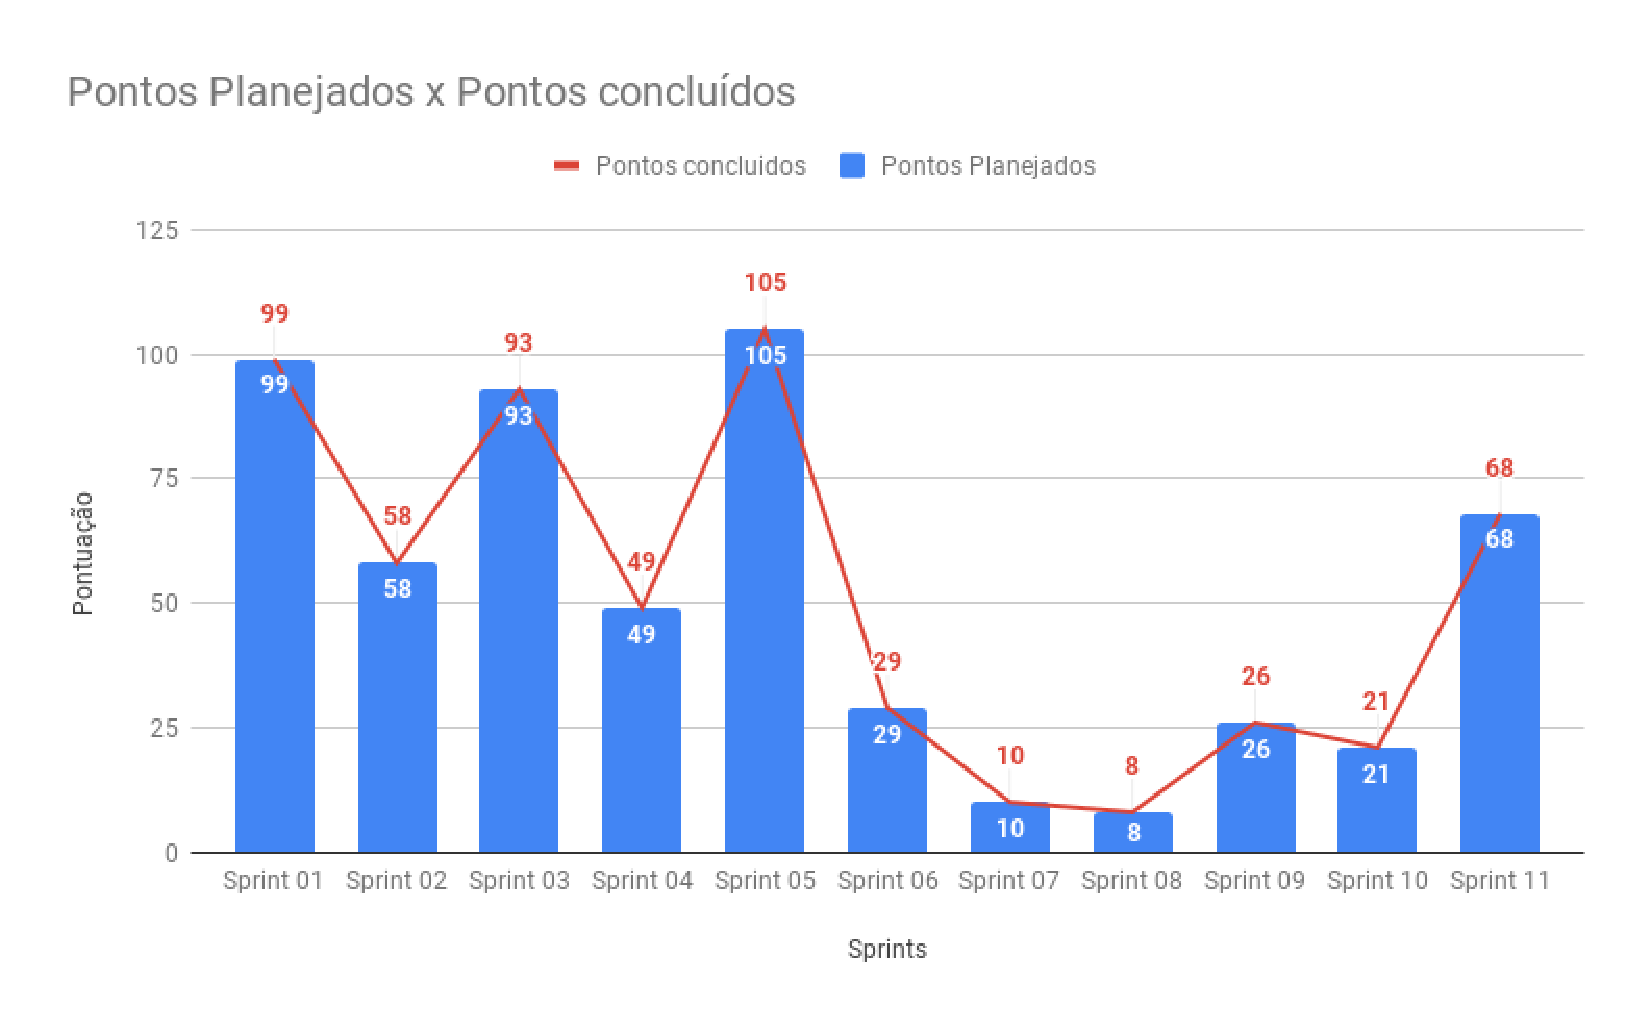
\includegraphics[keepaspectratio=true,scale=0.5]{figuras/pontos_planejados.eps}
  \caption[Pontos Planejados x Pontos Concluídos.]{Pontos Planejados x Pontos Concluídos. Fonte: Autor}
	\label{fig:planejamento}
\end{figure}

\begin{figure}[h!]
	\centering
  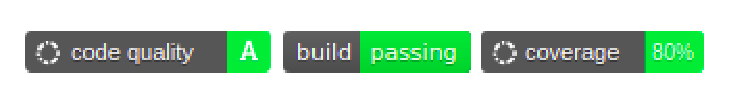
\includegraphics[keepaspectratio=true,scale=0.8]{figuras/build.eps}
  \caption[Build.]{Build. Fonte: Autor}
	\label{fig:build}
\end{figure}

\textbf{Resultado}: Como podemos ver, a build está funcionando perfeitamente e foi executado todos os pontos definidos
no planejamento do projeto.

\subsection{Objetivo 01: Qualidade de código}

\subsubsection{Questão 01: A qualidade do código está aceitável?}

\subsubsubsection{Métrica: Quantidade de issues geradas pela ferramenta de análise estática}

\begin{figure}[h!]
	\centering
  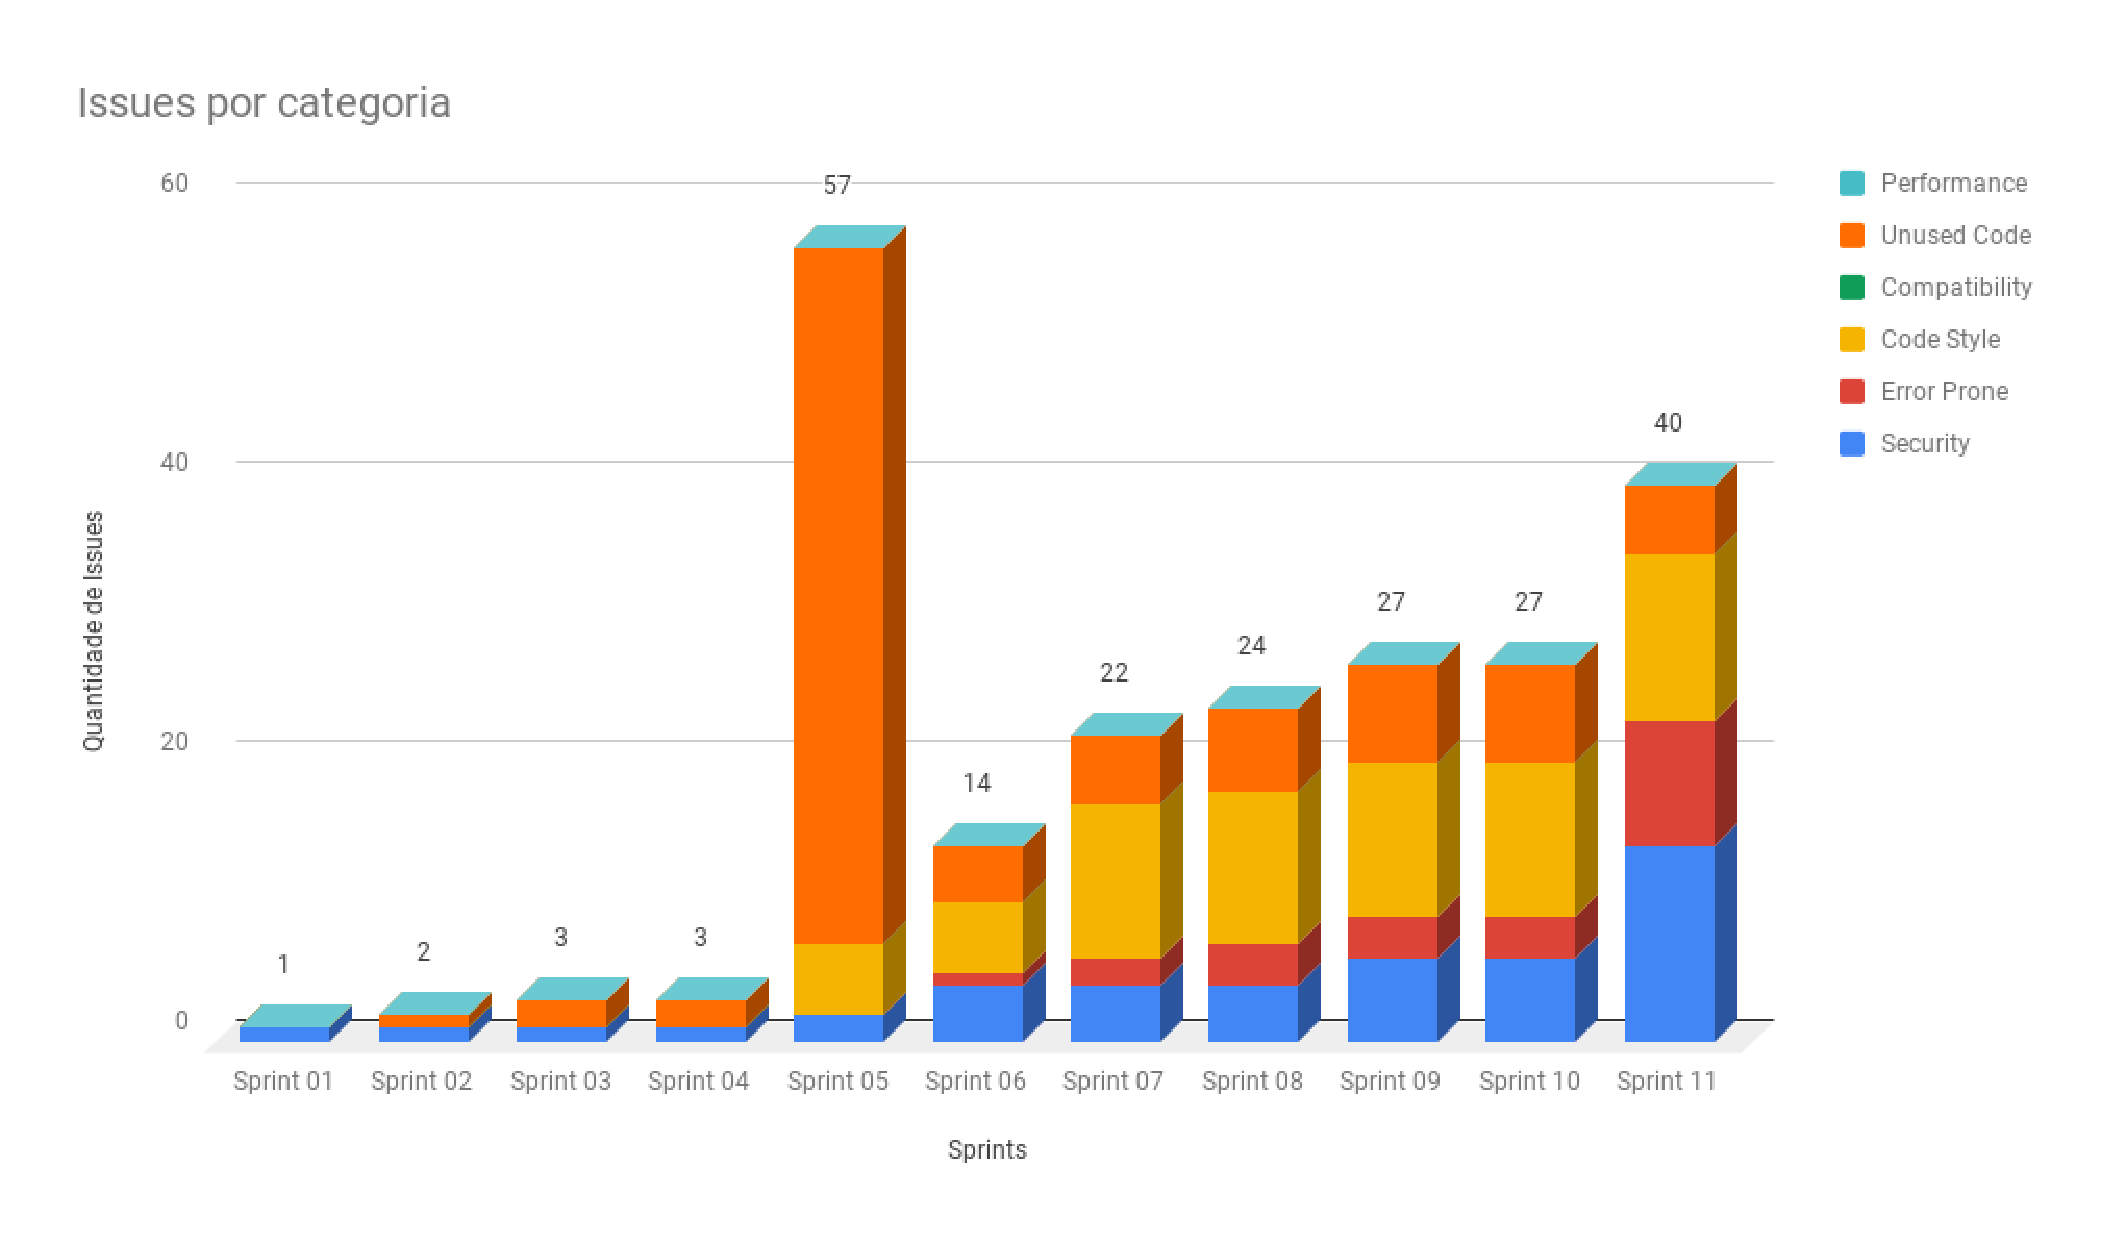
\includegraphics[keepaspectratio=true,scale=0.4]{figuras/issues_por_categoria.eps}
  \caption[Issues por Categoria.]{Issues por Categoria. Fonte: Autor}
	\label{fig:issues_categoria}
\end{figure}

\begin{itemize}
  \item \textbf{Descrição}: O resultado desta métrica será dado pela quantidade de issues que a ferramenta de análise estática de código encontrou, a ferramenta utiliza folhas de estilos normalmente adotadas para padronizar as linguagens, por exemplo a pep8 que é uma folha de estilo para a linguagem python padronizando seu código. Além disso cada issue é separado em categorias, entre elas as mais importantes são Style, Error Prone, Unused code, security.
  \item \textbf{Procedimentos}: Verificar a quantidade de issues por categoria geradas pela ferramenta de análise estática Codacy e o nível de gravidade de cada uma.
  \item \textbf{Análise}:
    \begin{itemize}
      \item \textbf{Valor Aceitável}: Menos de 50 issues, Refatorar sempre que possível o código até atingir o valor ótimo.
      \item \textbf{Valor Ótimo}: Nenhuma issue, Manter a qualidade do código estável.
      \item \textbf{Valor Preocupante}: Mais que 50 issues, Priorizar a refatoração do código com urgência utilizando de preferência folhas de estilo, e focar todos os esforços possíveis a fim de diminuir a quantidade de issues.
    \end{itemize}
  \item \textbf{Resultados}: Tivemos ao final do projeto apenas 40 Issues divididas em suas categorias, o que de acordo com a métrica é um valor aceitável.
\end{itemize}

\subsubsubsection{Métrica: Complexidade ciclomática}

\begin{figure}[h!]
	\centering
  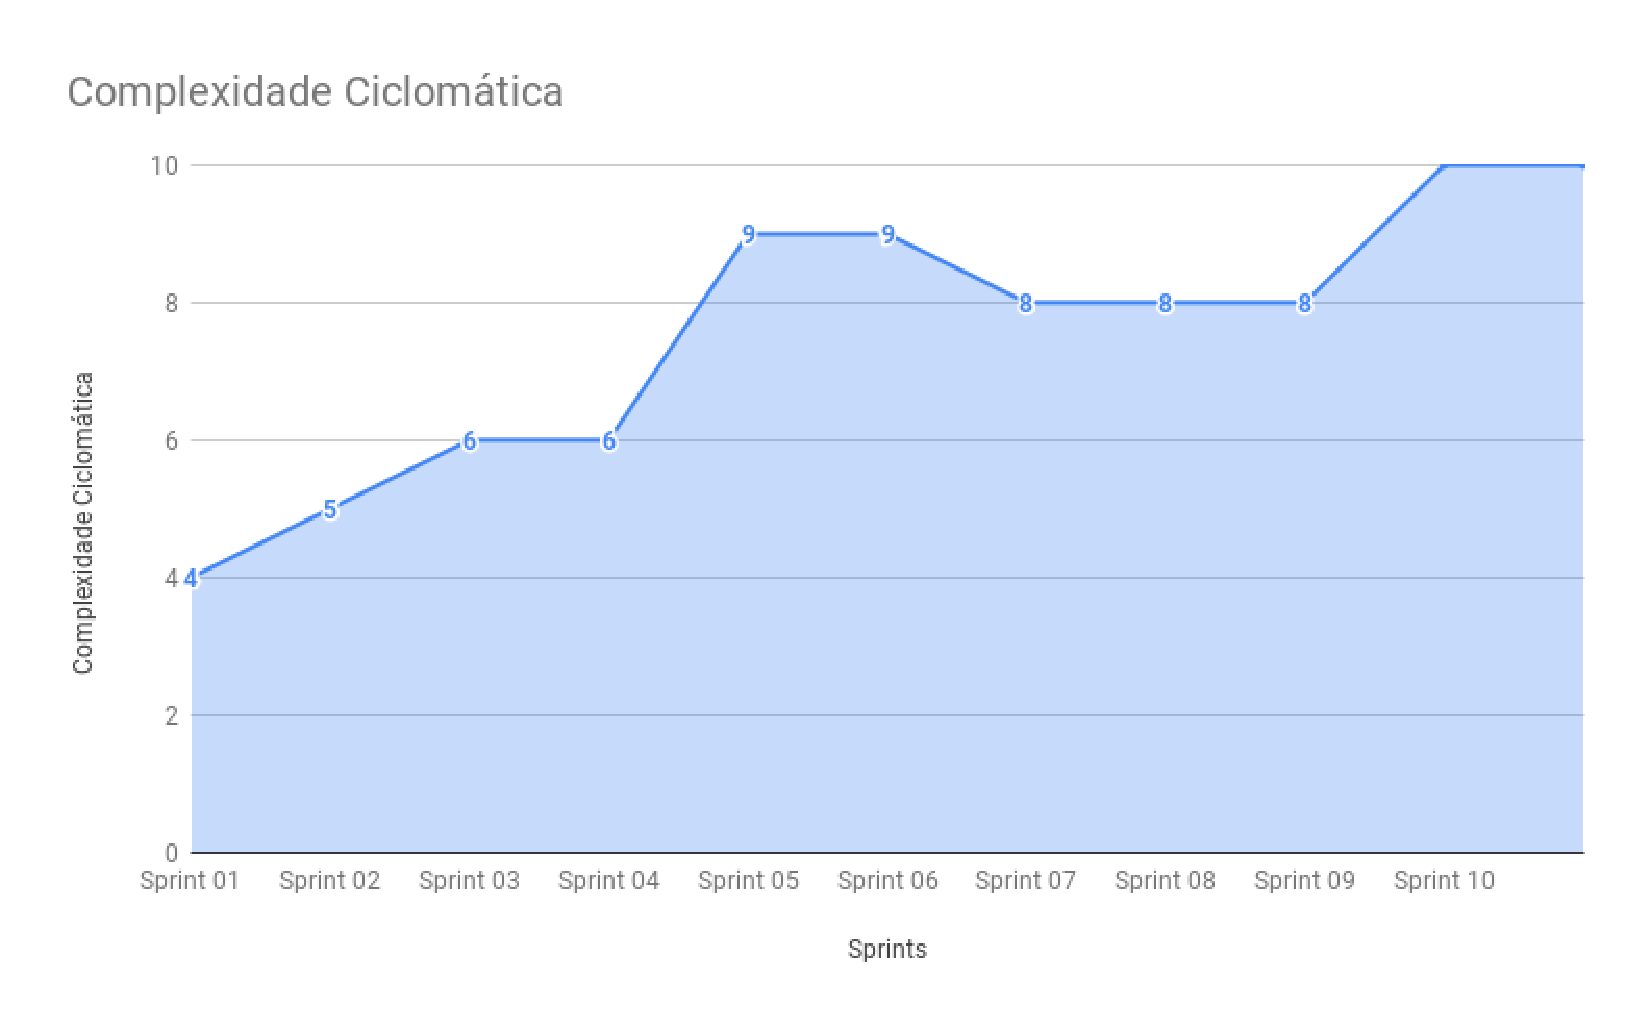
\includegraphics[keepaspectratio=true,scale=0.5]{figuras/complexidade_ciclomatica.eps}
  \caption[Complexidade Ciclomática.]{Complexidade Ciclomática. Fonte: Autor}
	\label{fig:complexidade}
\end{figure}

\begin{itemize}
  \item \textbf{Descrição}: O resultado desta métrica é realizado por meio de porcentagens, complexidade entre 0\% e 20\%, é um valor de ótimo para aceitável, complexidades acima de 20\%, gera complexidade computacional custosa podendo refletir em tempo de espera em consultas.
  \item \textbf{Procedimentos}: Na nova versão do Codacy a complexidade ciclomática do projeto vem em porcentagem.
  \item \textbf{Análise}:
    \begin{itemize}
      \item \textbf{Valor Aceitável}: Complexidade entre 5\% a 20\%, refatorar sempre que possível o código até atingir o valor ótimo.
      \item \textbf{Valor Ótimo}: Complexidade abaixo de 5\%, manter a qualidade do código estável.
      \item \textbf{Valor Preocupante}: Complexidade acima de 20\%, priorizar a refatoração do código com urgência, e focar todos os esforços possíveis a fim de aumentá-lo para o valor ótimo.
    \end{itemize}
  \item \textbf{Resultados}: Como podemos observar a complexidade ficou em torno de 10\%, ou seja, está com um valor de aceitável para ótimo.
\end{itemize}

\subsubsubsection{Métrica: Índice de qualidade (Certification)}

\begin{figure}[H]
	\centering
  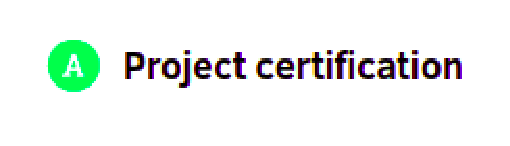
\includegraphics[keepaspectratio=true,scale=0.8]{figuras/certificado.eps}
  \caption[Certificação de Projeto.]{Certificação de Projeto. Fonte: Autor}
	\label{fig:certificacao}
\end{figure}

\begin{itemize}
  \item \textbf{Descrição}: O resultado desta métrica será dado em um índice entre F e A, onde F significa que o código está horrível, D significa que o código está ruim, C significa nota que o código está na média, B o código está bom e A o código está com uma qualidade excelente.
  \item \textbf{Procedimentos}: Verificar o índice de qualidade disponibilizado pela ferramenta codacy que indica a qualidade de código total de um projeto.
  \item \textbf{Análise}:
    \begin{itemize}
      \item \textbf{Valor Aceitável}: B e C, refatorar sempre que possível o código até atingir o valor ótimo.
      \item \textbf{Valor Ótimo}: A, manter a qualidade do código estável.
      \item \textbf{Valor Preocupante}: D e F, priorizar a refatoração do código com urgência, e focar todos os esforços possíveis a fim de aumentar esse índice.
    \end{itemize}
  \item \textbf{Resultados}: A qualidade do código sempre se manteve estável em nível ótimo.
\end{itemize}

\subsubsection{Questão 02: O software está com uma cobertura de código aceitável?}

\subsubsubsection{Métrica: Cobertura de Testes}

\begin{figure}[h!]
	\centering
  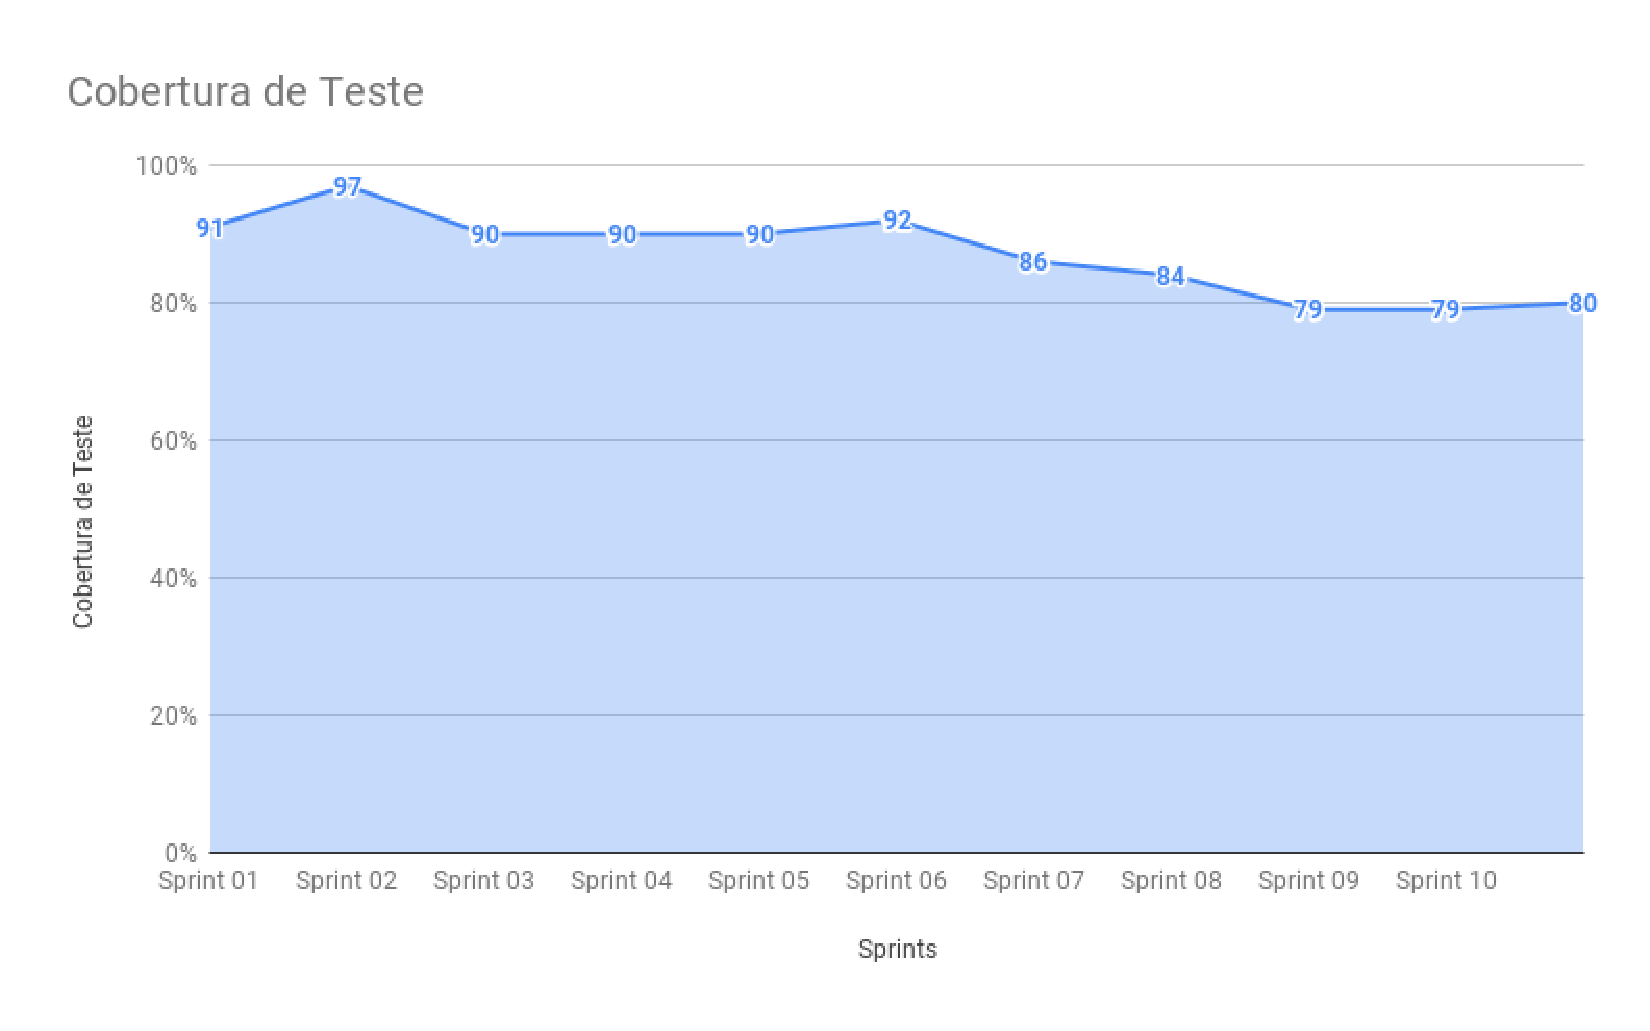
\includegraphics[keepaspectratio=true,scale=0.5]{figuras/cobertura_de_testes.eps}
  \caption[Cobertura de Testes.]{Cobertura de Testes. Fonte: Autor}
	\label{fig:testes}
\end{figure}

\begin{itemize}
  \item \textbf{Descrição}: O resultado desta métrica será dado em um valor de porcentagem que variará entre 0\% e 100\%, onde 0\% significa que nenhum dos arquivos analisados pela ferramenta foi testado e 100\% indica que todas as linhas de códigos forám testadas, mas não quer dizer que há uma cobertura completa de testes do software, ou seja, que testa todos os possíveis casos.
  \item \textbf{Procedimentos}: Foi verificado utilizando uma ferramenta de cobertura de teste chamada Codacy que rodará dentro do software, ela gera um tracking dos arquivos que necessitam de teste. Esse tracking demonstra uma porcentagem para cada arquivo, que indica a cobertura de testes deste e além disso indica a porcentagem total de cobertura do projeto.
  \item \textbf{Análise}:
    \begin{itemize}
      \item \textbf{Valor Aceitável}: Maior que 50\% de cobertura de código, a medida a ser tomada é manter o nível de cobertura, e se possível aumentar o nível para que este alcance o valor ótimo.
      \item \textbf{Valor Ótimo}: Maior que 90\% de cobertura de código, a medida a ser tomada é manter o nível de cobertura e tentar alcançar o 100\%.
      \item \textbf{Valor Preocupante}: Menor que 50\% de cobertura de código, a medida a ser tomada é priorizar cobertura de testes como um fator crítico na equipe, e focar todos os esforços possíveis a fim de aumentar o nível de cobertura
    \end{itemize}
  \item \textbf{Resultados}: Cobertura de código final é de 80\% ou seja um valor aceitável. Com isso podemos concluir que a qualidade do código está boa.
\end{itemize}

\subsection{Objetivo 02: Conhecimento da equipe}

\subsubsection{Questão 01: A equipe tem conhecimento suficiente para o desenvolvimento?}

\subsubsubsection{Métrica: Quadro de conhecimento}

\begin{figure}[h!]
	\centering
  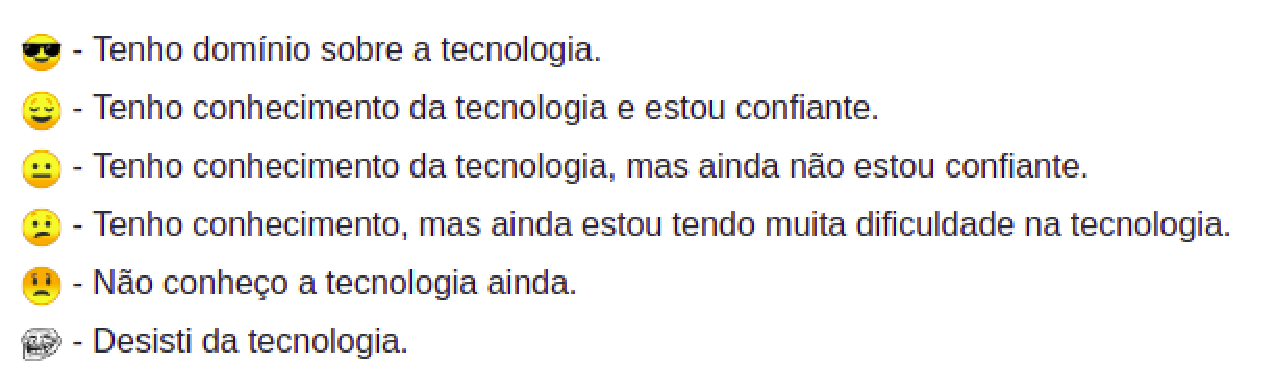
\includegraphics[keepaspectratio=true,scale=0.6]{figuras/conhecimento_lista.eps}
  \caption[Conhecimentos.]{Conhecimentos. Fonte: Autor}
	\label{fig:conhecimentos}
\end{figure}

\begin{figure}[h!]
	\centering
  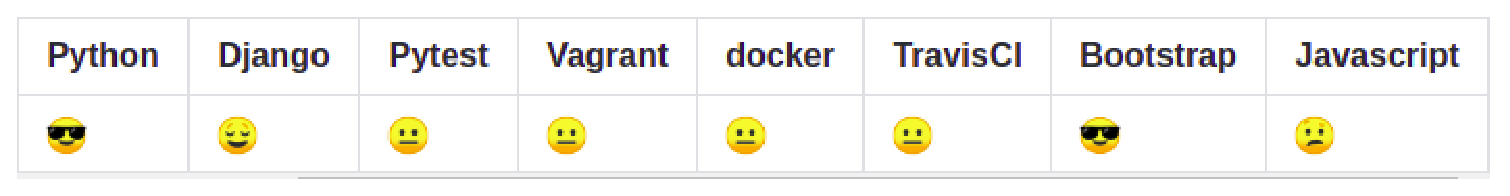
\includegraphics[keepaspectratio=true,scale=0.6]{figuras/conhecimento_inicio.eps}
  \caption[Conhecimentos Inicio.]{Conhecimentos Inicio. Fonte: Autor}
	\label{fig:conhecimentos_inicio}
\end{figure}

\begin{figure}[h!]
	\centering
  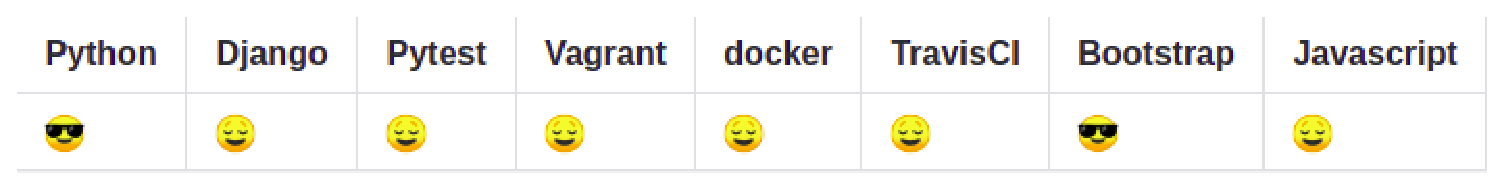
\includegraphics[keepaspectratio=true,scale=0.6]{figuras/conhecimento_final.eps}
  \caption[Conhecimentos Final.]{Conhecimentos Final. Fonte: Autor}
	\label{fig:conhecimentos_final}
\end{figure}

\begin{itemize}
  \item \textbf{Descrição}: O resultado desta métrica será dado no quadro de conhecimento, na qual o eixo x será as tecnologias empregadas no projeto e o eixo y será o nome dos integrantes da equipe, terá seis rostos que dirá se o integrante tem domínio da tecnologia, está aprendendo e consegue se virar sozinho, está tendo dificuldades na tecnologia ou se desistiu da tecnologia.
  \item \textbf{Procedimentos}: Verificar como está o quadro de conhecimento a cada sprint e identificar as tecnologias
    que os desenvolvedores estão tendo mais dificuldade de aprender.
  \item \textbf{Análise}:
    \begin{itemize}
      \item \textbf{Valor Aceitável}: "Tenho conhecimento da tecnologia, mas ainda não estou confiante". Estudar a tecnologia sempre que houver tempo.
      \item \textbf{Valor Ótimo}: "Tenho conhecimento da tecnologia e estou confiante ou tenho domínio sobre a tecnologia". Manter o domínio sobre a tecnologia.
      \item \textbf{Valor Preocupante}: "Tenho dificuldade ou não tenho conhecimento sobre a tecnologia". Criar dojos e estudar a tecnologia mais a fundo com a equipe.
      \item \textbf{Desistência}: Encontrar outra tecnologia para substituí-la na função que ela ia desempenhar.
    \end{itemize}
  \item \textbf{Resultados}: Ao final do projeto o desenvolvedor teve um valor ótimo de domínio das tecnologias utilizadas, ocasionando na finalização do software.
\end{itemize}
